\documentclass{beamer}
\usepackage{graphicx}
\usepackage{xcolor}
\usepackage{mathtools}
\usetheme[titlepagelogo=img/firenze,% Logo for the first page
		  language=italian,
		  bullet=circle,
		  color=blue,
         ]{TorinoTh}
\usepackage[beamer,customcolors]{hf-tikz}
\usepackage[section]{placeins}
\usepackage{booktabs}

\definecolor{UniBlue}{RGB}{83,121,170}
\uselanguage{italian}
\languagepath{italian}
\setbeamercolor{block title}{use=structure,fg=white,bg=UniBlue}
\setbeamercolor{block body}{use=structure,fg=black,bg=white}

\author{}
\rel{{\normalsize \emph{Machine Learning}}\\\vspace{0.3cm}Saverio Meucci}
\title{\huge Harnessing adversarial examples}
\date{10 Gennaio 2017}

\begin{document}

\titlepageframe
\begin{frame}{Introduction}

For this project, a model for a multi-label problem is trained, using the MNIST dataset. Once the model is obtained, adversarial examples can be generated. An adversarial example is an example that is only slightly different from the original and correctly classified example that a model misclassify with a high confidence.

\vspace{0.1in}

The objective of this project is to harness adversarial examples to train a more robust model, by lowering the classification error and the confidence associated with those misclassifications.

\end{frame}


\section{Dataset}

The MNIST dataset is a large dataset of handwritten digits, thus including ten mutually exclusive classes. It was creates from the samples of the NIST dataset; the originally black and white images were normalized to fit 28x28 pixels images and anti-alisiasing were used, which introduced grayscale levels, so that the pixel values are in the range [0, 255].

The MNIST dataset contains 60,000 training images (divided in two sets, train and validation, with 55,000 and 5,000 images resprectively) and 10,000 testing images.

For this project, from each sample the mean image of the dataset were subtracted.
\begin{tframe}{Explaining adversarial examples}



\end{tframe}

%%--------------------------------------------%%

\begin{tframe}{Generating adversarial examples}

Let $\theta$ be the parameters of a model, x the input to the model, y the targets associated with x (for machine learning tasks that have targets) and $J(\theta, x, y)$ be the cost used to train the neural network. 
We can linearize the cost function around the current value of $\theta$, obtaining an optimal max-norm constrained pertubation of ,

$$ \eta = \epsilon * sign(\nabla_x J(\theta, x, y)) $$

The adversarial examples can thus be obtained as follow,

$$ x = x + \eta $$


\end{tframe}
\begin{tframe}{CNN - Architecture}

The net is based on LeNet and consists of eight layers, as shown in the following image.

\begin{figure}[h]
	\begin{center}
		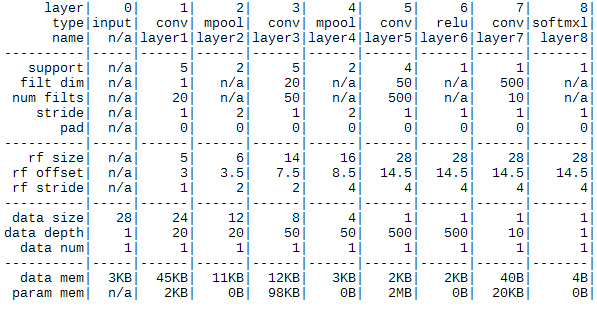
\includegraphics[width=1\textwidth]{img/cnn.png}
	\end{center}
	\label{fig:cnn}
\end{figure}

\end{tframe}

\begin{tframe}{CNN - Settings}

\vspace{0.1in}
\vspace{0.1in}
\vspace{0.1in}

\begin{itemize}
\item Number of epochs 30
\item Learning rate initialized to 0.001
\item Softmax log-loss as a cost function
\item SGD with momentum initialized to 0.9
\item Weight decay of 0.0005
\end{itemize}


\end{tframe}
\section{Standard Training}

The net was trained in a standard way, using the 60,000 images of the train and validation sets. The training went on for 30 epochs.

\begin{center}
  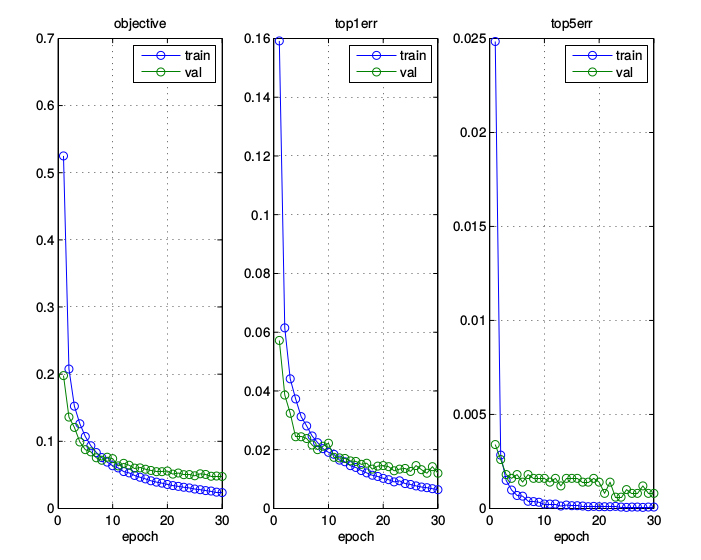
\includegraphics[width=0.7\textwidth]{img/train-base.png}
	\label{train-base} 
\end{center}

The tests carried out on the trained model were of two kind. The first test was made using the 10,000 clean samples from the testing set; the second test was made using the adversarial examples, that is the same samples as the first test but with an added perturbation computed as shown in Section 0.4.

\begin{table}[h]
\centering
\begin{tabular}{@{}lll@{}}
\toprule
                               & Clean & Adversarial \\ \midrule
Correctly Predicted            & 98.47 & 3.36        \\
Error                          & 1.53  & 96.64       \\
Confidence                     & 98.59 & 93.82       \\
Confidence Correctly Predicted & 99.04 & 91.67       \\
Confidence Error               & 69.95 & 93.89       \\ \bottomrule
\end{tabular}
\caption{Test results for standard training model.}
\label{standard-test}
\end{table}
\FloatBarrier


As we can see from the results shown in Table~\ref{standard-test}, the classification using the clean samples as test images worked great, with high prediction rate and confidence. The results for the adversarial test, however, behaved as expected, with a large percentage of misclassification with a high confidence.
\begin{tframe}{Mixed Training}

For this case, adversarial examples were included in the training phase. At each epoch, the adversarial example of each image was computed, given the model at that particular epoch. 

\vspace{0.1in}

Both images, clean and adversarial, were used in the training process, similar to dataset augmentation. This way, both the clean examples and the adversarial examples participate in the optimization of the parameters of the model in order to decrease the loss.

\vspace{0.1in}

Adversarial examples are thus generated dynamically at each epoch, so that the model is trained considering its blind-spots.

\end{tframe}

\begin{tframe}{Mixed Training}

\begin{center}
  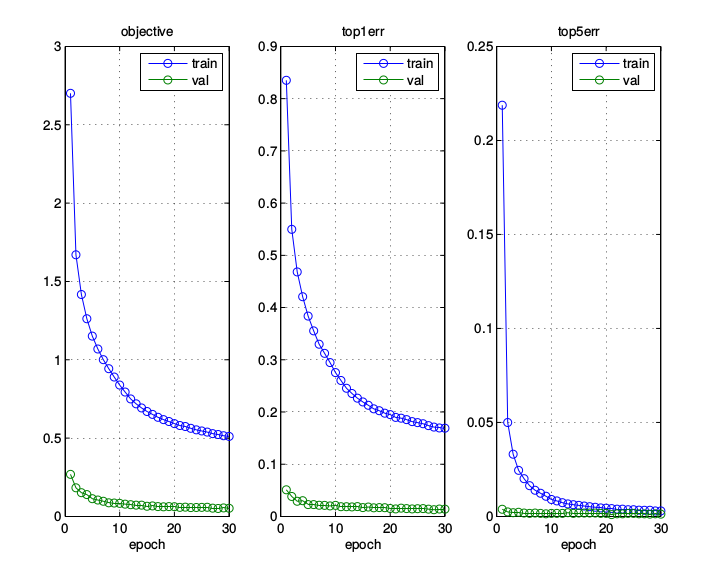
\includegraphics[width=0.7\textwidth]{img/train-mix.png}
	\label{train-mix} 
\end{center}

\end{tframe}

\begin{tframe}{Mixed Training}

The tests were carried out as for the standard training.

\begin{table}[h]
\centering
\begin{tabular}{@{}lll@{}}
\toprule
                               & Clean & Adversarial \\ \midrule
Correctly Predicted            & 98.21 & 85.28       \\
Error                          & 1.79  & 14.72       \\
Confidence                     & 97.29 & 86.30       \\
Correctly Predicted Confidence & 97.85 & 89.07       \\
Error Confidence               & 66.91 & 70.22       \\ \bottomrule
\end{tabular}
\end{table}

\end{tframe}
\begin{tframe}{Adversarial Training}

The method of training used for this case follows the one proposed by [1].

\vspace{0.1in}

The objective function is modified to include adversarial examples in the training phase:

$$ 	\tilde{J}(\theta, x, y) = \alpha J(\theta, x, y) + ( 1 - \alpha)J(\theta, x + \epsilon sign(\nabla_{x}J(\theta, x, y)), y) $$

\end{tframe}

\begin{tframe}{Adversarial Training}

\begin{center}
  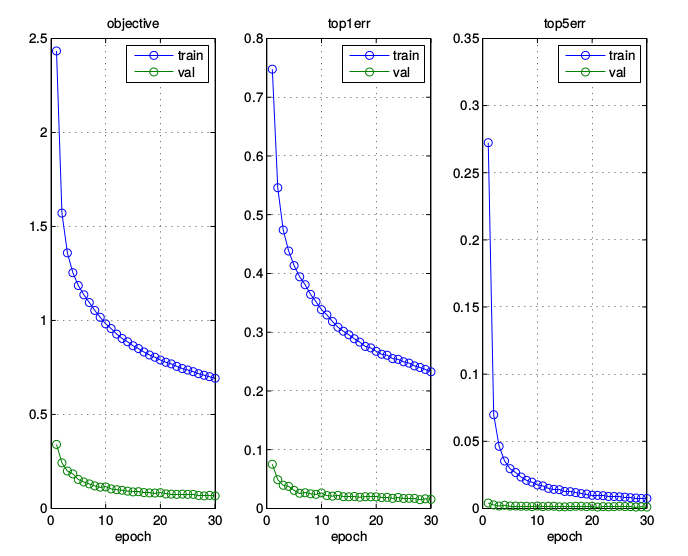
\includegraphics[width=0.7\textwidth]{img/train-adv.png}
	\label{train-mix} 
\end{center}

\end{tframe}

\begin{tframe}{Adversarial Training}

The tests were carried out as for the standard and mixed training.

\begin{table}[h]
\centering
\begin{tabular}{@{}lll@{}}
\toprule
                               & Clean & Adversarial \\ \midrule
Correctly Predicted            & 97.97 & 77.80       \\
Error                          & 2.03  & 22.20       \\
Confidence                     & 96.03 & 79.05       \\
Confidence Correctly Predicted & 96.69 & 82.55       \\
Confidence Error               & 64.23 & 66.79       \\ \bottomrule
\end{tabular}
\end{table}

\end{tframe}
\begin{tframe}{References}

[1] I. J. Goodfellow, J. Shlens and C. Szegedy, "Explaining and harnessing adversarial examples", arXiv preprint arXiv:1412.6572, 2014

\vspace{0.1in}

\end{tframe}

\end{document}